% Import default values & document settings
% Layout settings
\newcommand{\FIITdefaultFontSize}[0] {12pt}
\setcounter{secnumdepth}{3}
\setcounter{tocdepth}{3}

% Language settings
\newcommand{\FIITlanguage}[0] {slovak}
% \newcommand{\FIITlanguage}[0] {slovak,english}
%\def\FIITlagEN{}

% Global texts
\newcommand{\FIITuniversity}[0] {Slovak University of Technology in Bratislava}
\newcommand{\FIITuniversitySK}[0] {Slovenská technická univerzita v Bratislave}
\newcommand{\FIITfaculty}[0] {Faculty of informatics and information technologies}
\newcommand{\FIITfacultySK}[0] {Fakulta informatiky a informačných technológií}
\newcommand{\FIITthesis}[0] {Bachelor's thesis}
\newcommand{\FIITthesisSK}[0] {Bakalárska práca}
\newcommand{\FIITtitle}[0] {Research in the field of Digital Twin technology}
\newcommand{\FIITtitleSK}[0] {Výskum v oblasti technológie digitálneho dvojčaťa}
\newcommand{\FIITauthor}[0] {Dávid Truhlář}
\newcommand{\FIITsupervisor}[0] {Ing. Matej Petrík}
\newcommand{\FIITevidenceNumber}[0] {FIIT-16768-120897}
\newcommand{\FIITdate}[0] {May 2025}
\newcommand{\FIITdateSK}[0] {Máj 2025}
\newcommand{\FIITstudyProgram}[0] {Informatics}
\newcommand{\FIITstudyProgramSK}[0] {Informatika}
\newcommand{\FIITstudyField}[0] {Computer Science}
\newcommand{\FIITdegreeCourseSK}[0] {Informatika}
\newcommand{\FIITinstitute}[0] {Institute of Computer Engineering and Applied Informatics}
\newcommand{\FIITinstituteSK}[0] {Ústav počítačového inžinierstva a aplikovanej informatiky}
\newcommand{\FIITsignPlace}[0] {In Bratislava, }
\newcommand{\FIITsignPlaceSK}[0] {V Bratislave, }
\newcommand{\FIITsignDate}[0] {8.2.2025}
\newcommand{\FIITArchiveName}[0] {BP\_prilohy\_digital\_JanoMrkvicka.zip}


% Setup document
\documentclass[\FIITdefaultFontSize,a4paper,twoside,openright,\FIITlanguage]{book}

% Load all necessary packages
\usepackage[final]{pdfpages}
\usepackage[utf8]{inputenc}
\usepackage[T1]{fontenc}
\usepackage[\FIITlanguage]{babel}
\usepackage[a4paper]{geometry}
\usepackage[
    left = \glqq,% 
    right = \grqq,% 
    leftsub = \glq,% 
    rightsub = \grq%
]{dirtytalk}
\usepackage[parfill]{parskip}
\usepackage{enumitem}
\usepackage{calc}
\usepackage{graphicx}
\usepackage{float}
\usepackage{longtable}
\usepackage{setspace}
\usepackage{tabularx}
\usepackage{fancyhdr}
\usepackage[backend=bibtex,sorting=none]{biblatex}
\usepackage{listings}
\usepackage{lscape}
\usepackage{afterpage}
\usepackage{hyperref}
%\usepackage{bera}
\usepackage{listings}
\usepackage{xcolor}
\usepackage{lipsum}
\usepackage{minted}
\usepackage{tikz}
\usepackage{tocloft}
\usepackage{comment}
\usepackage{titlesec}


% Remove unnecessary gap between paragraph if large figure is inserted after them
\raggedbottom

% lscape.sty Produce landscape pages in a (mainly) portrait document.
\usepackage{lscape}

% Custom commands
\newcommand{\signaturespace}[2]{
  % #1 = width of the dotted line
  % #2 = legend
  \begingroup
  \renewcommand{\arraystretch}{0}
  \begin{tabular}[t]{cc}
  \hspace*{0pt}
  \cleaders\hbox{\kern.6pt.\kern.6pt}\hskip#1\relax
  \hspace*{0pt}
  \\[0.5cm]
  #2
  \end{tabular}
  \endgroup
}

\newcommand{\emptypage}{\newpage
\thispagestyle{empty}
\mbox{}
\newpage}

% openright does not work :(
\let\tmp\oddsidemargin
\let\oddsidemargin\evensidemargin
\let\evensidemargin\tmp
\reversemarginpar

\titleformat{\chapter}[hang]
  {\normalfont\huge\bfseries} 
  {\thechapter\quad}         
  {0pt}                      
  {}                          

% Setup bibliography
\bibliography{bibliography}

% Page design
\pagestyle{fancy}
\lhead{\nouppercase{\leftmark}}
\chead{}
\rhead{}
\lfoot{}
\cfoot{\thepage}
\rfoot{}

\begin{document}

% Initialize document
% Layout
\setstretch{1.5}

% Bibliography
\ifx\FIITlagEN\undefined
\defbibheading{references}[Zoznam použitej literatúry]{ 
  \chapter*{#1}
  \addcontentsline{toc}{chapter}{#1}
  \markboth{#1}{#1}
}
\defbibheading{referencessec}[Zoznam použitej literatúry]{ 
  \section*{#1}
  \markboth{#1}{#1}
}
\else
\defbibheading{references}[References]{ 
  \chapter*{#1}
  \addcontentsline{toc}{chapter}{#1}
  \markboth{#1}{#1}
}
\defbibheading{referencessec}[References]{ 
  \section*{#1}
  \markboth{#1}{#1}
}
\fi

% Syntax highlighting
\setminted[]{linenos,tabsize=2,breaklines}
\colorlet{punct}{red!60!black}
\definecolor{background}{HTML}{EEEEEE}
\definecolor{delim}{RGB}{20,105,176}
\colorlet{numb}{magenta!60!black}

% Text highlighting
\makeatletter
\newenvironment{btHighlight}[1][]
{\begingroup\tikzset{bt@Highlight@par/.style={#1}}\begin{lrbox}{\@tempboxa}}
{\end{lrbox}\bt@HL@box[bt@Highlight@par]{\@tempboxa}\endgroup}

\newcommand\btHL[1][]{%
  \begin{btHighlight}[#1]\bgroup\aftergroup\bt@HL@endenv%
}
\def\bt@HL@endenv{%
  \end{btHighlight}%   
  \egroup
}
\newcommand{\bt@HL@box}[2][]{%
  \tikz[#1]{%
    \pgfpathrectangle{\pgfpoint{1pt}{0pt}}{\pgfpoint{\wd #2}{\ht #2}}%
    \pgfusepath{use as bounding box}%
    \node[anchor=base west, fill=black!10,outer sep=0pt,inner xsep=1pt, inner ysep=-2pt, rounded corners=3pt, minimum height=\ht\strutbox+1pt,#1]{\raisebox{1pt}{\strut}\strut\usebox{#2}};
  }%
}
\makeatother

% Cover & title page
% Cover page
	\begin{center}
\thispagestyle{empty}
\ifx\FIITlagEN\undefined
{\Large \FIITuniversitySK}
\else
{\Large \FIITuniversity}
\fi
\par\end{center}{\Large \par}

\begin{center}
\ifx\FIITlagEN\undefined
{\Large \FIITfacultySK}
\else
{\Large \FIITfaculty}
\fi
\par\end{center}{\Large \par}

\smallskip{}

\begin{center}
\ifx\FIITlagEN\undefined
Evidenčné číslo: \FIITevidenceNumber
\else
Reg. No.: \FIITevidenceNumber
\fi
\par\end{center}
\vfill{}

\begin{center}
\textbf{\Large \FIITauthor}
\par\end{center}{\Large \par}

\medskip{}


\begin{center}
\ifx\FIITlagEN\undefined
\textbf{\LARGE \FIITtitleSK}
\else
\textbf{\LARGE \FIITtitle}
\fi
\par\end{center}{\huge \par}

\medskip{}


\begin{center}

\ifx\FIITlagEN\undefined
{\Large \FIITthesisSK}
\else
{\Large \FIITthesis}
\fi
\par\end{center}{\Large \par}

\vfill{}

\ifx\FIITlagEN\undefined
Vedúci záverečnej práce: \FIITsupervisor
\else
Thesis supervisor: \FIITsupervisor
\fi

\medskip{}

\ifx\FIITlagEN\undefined
\FIITdateSK
\else
\FIITdate
\fi

\pagenumbering{roman}
\emptypage





% Thesis title page
	\begin{center}
\thispagestyle{empty}
\ifx\FIITlagEN\undefined
{\Large \FIITuniversitySK}
\else
{\Large \FIITuniversity}
\fi
\par\end{center}{\Large \par}

\begin{center}
\ifx\FIITlagEN\undefined
{\Large \FIITfacultySK}
\else
{\Large \FIITfaculty}
\fi
\par\end{center}{\Large \par}

\smallskip{}

\begin{center}
\ifx\FIITlagEN\undefined
Evidenčné číslo: \FIITevidenceNumber
\else
Reg. No.: \FIITevidenceNumber
\fi
\par\end{center}
\vfill{}

\begin{center}
\textbf{\Large \FIITauthor}
\par\end{center}{\Large \par}

\medskip{}


\begin{center}
\ifx\FIITlagEN\undefined
\textbf{\LARGE \FIITtitleSK}
\else
\textbf{\LARGE \FIITtitle}
\fi
\par\end{center}{\huge \par}

\medskip{}


\begin{center}

\ifx\FIITlagEN\undefined
{\Large \FIITthesisSK}
\else
{\Large \FIITthesis}
\fi
\par\end{center}{\Large \par}

\vfill{}

\ifx\FIITlagEN\undefined
Študijný program: \FIITstudyProgramSK

Študijný odbor: \FIITdegreeCourseSK

Školiace pracovisko: \FIITinstituteSK

Vedúci záverečnej práce: \FIITsupervisor
\else
Study programme: \FIITstudyProgram

Study field: \FIITstudyField

Training workplace: \FIITinstitute

Thesis supervisor: \FIITsupervisor
\fi

\medskip{}

\ifx\FIITlagEN\undefined
\FIITdateSK
\else
\FIITdate
\fi

\emptypage


% Thesis assignment
\newpage
\thispagestyle{empty}
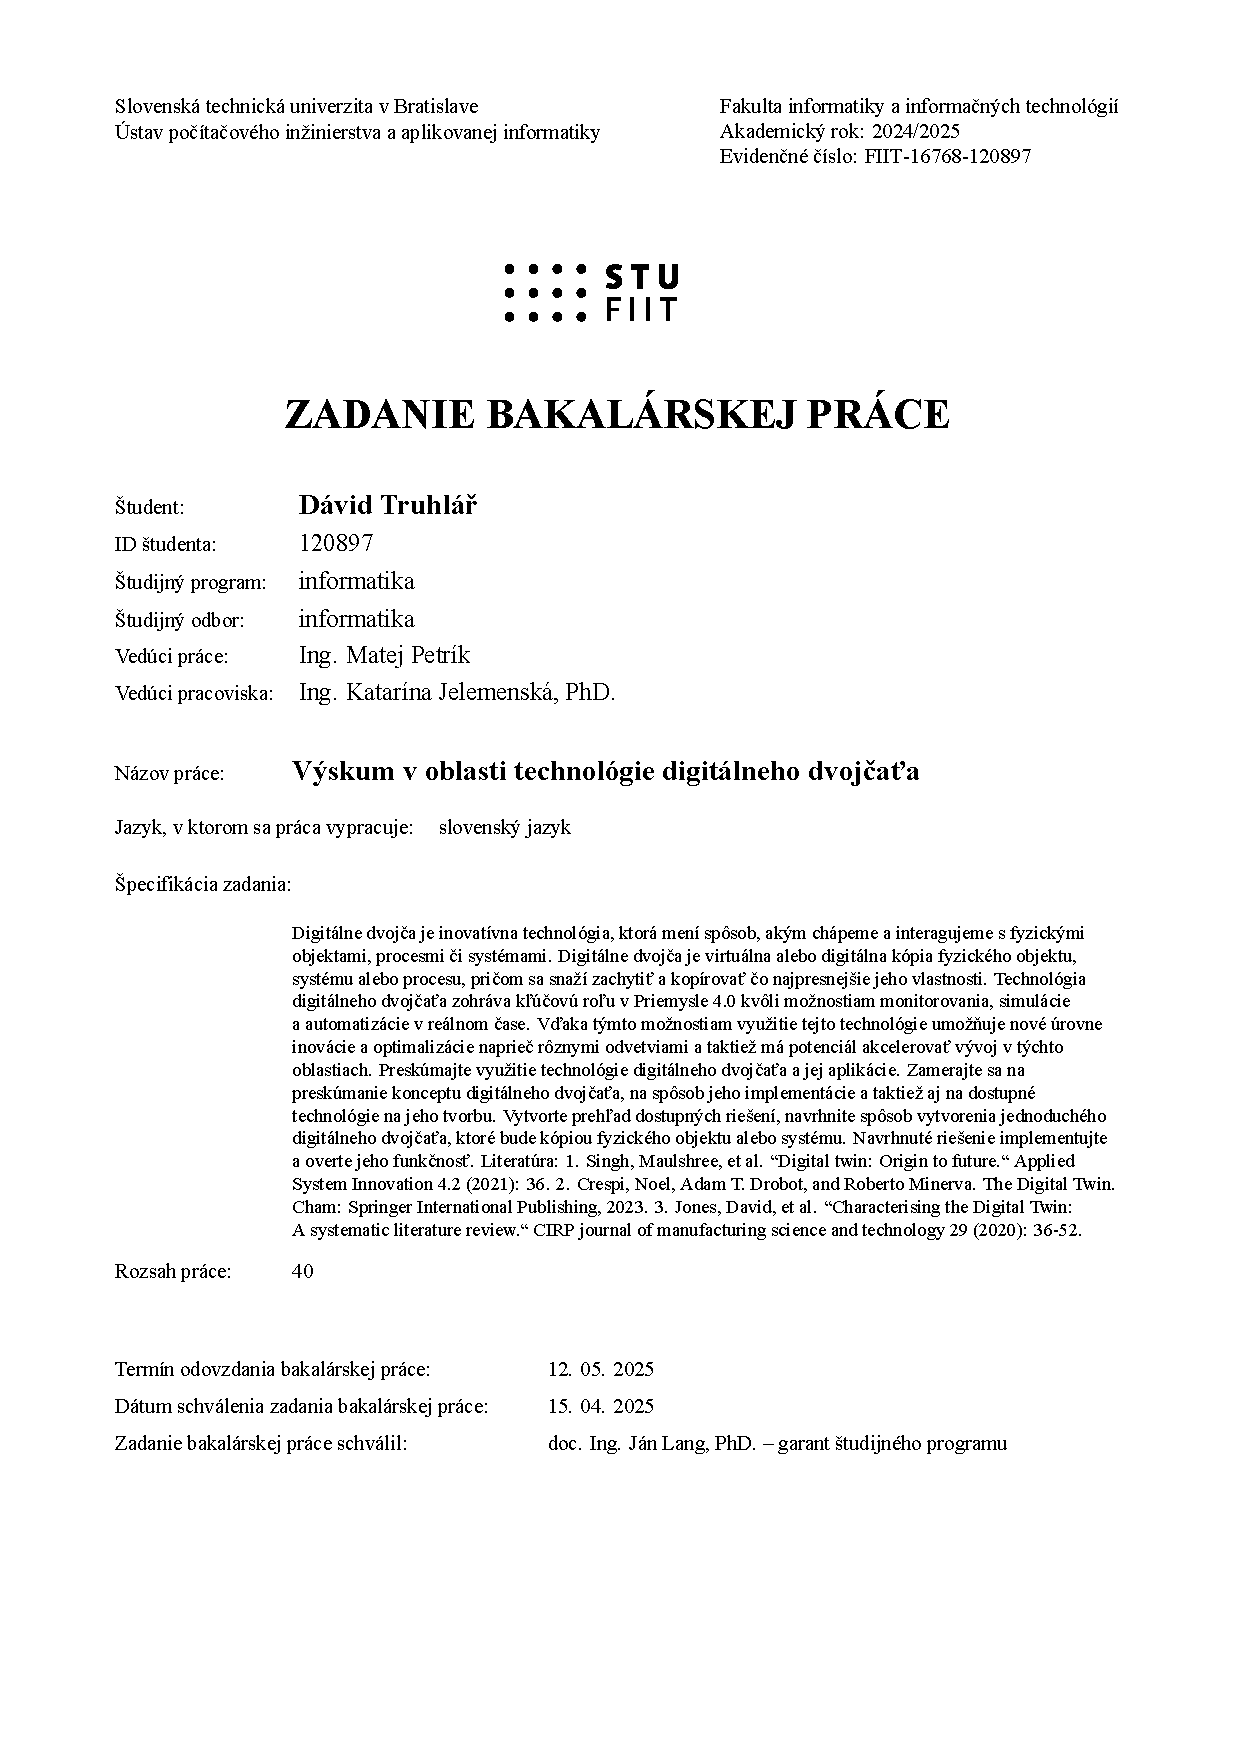
\includepdf[pages=1,scale=0.85]{assets/zadanie.pdf}
\newpage
%\emptypage

% Declaration of honor
\thispagestyle{empty}

\vspace*{\fill}

\ifx\FIITlagEN\undefined
\section*{Čestné prehlásenie}
\else
\section*{Declaration of honor}
\fi
\par{
Čestne vyhlasujem, že som túto prácu vypracoval samostatne, na základe konzultácií a s použitím uvedenej literatúry.
\\ 
\\
}
\ifx\FIITlagEN\undefined
\FIITsignPlaceSK \FIITsignDate
\else
\FIITsignPlace \FIITsignDate
\fi
\hspace*{\fill} \signaturespace{5cm}{\FIITauthor}

\emptypage

% Acknowledgements - Poďakovanie
%\thispagestyle{empty}

\vspace*{\fill}

\ifx\FIITlagEN\undefined
\section*{Poďakovanie}
\else
\section*{Special thanks}
\fi

\lipsum[1]

\emptypage

% Annotation
% % Annotation in Slovak
\thispagestyle{empty}

\vspace*{\fill}

\section*{Anotácia}

\begin{minipage}[t]{1\columnwidth}
\FIITuniversitySK

\FIITfacultySK

Študijný program: \FIITstudyProgramSK\\

Autor: \FIITauthor

\FIITthesisSK: \FIITtitleSK

Vedúci projektu: \FIITsupervisor

\FIITdateSK
\end{minipage}

\bigskip{}

\lipsum[2]

\newpage{}\thispagestyle{empty}\medskip{}

\emptypage

% Annotation in English
\thispagestyle{empty}

\vspace*{\fill}

\section*{Annotation}

\begin{minipage}[t]{1\columnwidth}
\FIITuniversity

\FIITfaculty

Degree Course: \FIITstudyProgram\\

Author: \FIITauthor

\FIITthesis: \FIITtitle

Supervisor: \FIITsupervisor

\FIITdate
\end{minipage}

\bigskip{}

\lipsum[1]

\newpage{}\thispagestyle{empty}

\emptypage

% Table of contents
\ifx\FIITlagEN\undefined
\renewcommand{\contentsname}{Obsah}
\else
\renewcommand{\contentsname}{Table of contents}
\fi
\tableofcontents{}
%\emptypage

% List of figures - Zoznam obrázkov
\listoffigures
%\emptypage

% List of tables
%\listoftables
%\emptypage

% List of abbreviations
\thispagestyle{plain}

\ifx\FIITlagEN\undefined
\section*{\Huge Zoznam použitých skratiek}
\markboth{Zoznam použitých skratiek}{Zoznam použitých skratiek}
\else
\section*{\Huge List of abbreviations used}
\markboth{List of abbreviations used}{List of abbreviations used}
\fi
\vskip 1cm

\begin{tabular}{ >{\bfseries}m{2cm} m{10cm} }
BP      & Bakalárska práca \\
DT      & Digitálne dvojča \\
IoT     & Internet vecí\\
ML      & Strojové učenie \\
RAN     & Rádiová prístupová sieť \\
UE      & Užívateľské zariadenie \\
GDPR    & Všeobecné nariadenie o ochrane údajov \\
\begin{comment}
API		& Application Programming Interface \\
CSV		& Comma-Separated Values \\
DNS		& Domain Name System \\
HTTP	& Hyper-Text Transfer Protocol \\
IMAP	& Internet Message Access Protocol \\
IP		& Internet Protocol \\
JSON	& JavaScript Object Notation \\
MySQL	& Maria SQL  \\
OS		& Operating System \\
POP3    & Post Office Protocol, version 3\\
REST    & Representational state transfer \\
SMTP	& Simple Mail Transfer Protocol \\
SQL		& Structured Query Language \\
TLS     & Transport Layer Security \\
URL		& Unified Resource Locator \\
XML		& Extensible Markup Language  
\end{comment}
\end{tabular}

\emptypage

% Enable page numbering
\pagenumbering{arabic}

% Begin refferences segment
\begin{refsegment}

%\chapter{Technický abstrakt}

Siete piatej generácie (5G) predstavujú základnú infraštruktúru pre aplikácie s prísnymi požiadavkami na odozvu (latency) a spoľahlivosť. Technológia digitálneho dvojčaťa  (DT) má v tomto kontexte potenciál slúžiť ako adaptívna vrstva pre simuláciu, monitorovanie a klasifikáciu sieťovej prevádzky. Táto práca sa zameriava na návrh a implementáciu DT 5G siete, ktoré v reálnom čase analyzuje metriky jadra siete a klasifikuje aktuálny typ prevádzky pomocou rekurentných neurónových sietí (LSTM).

Navrhnuté DT pozostáva z kontajnerizovaného simulačného prostredia založeného na Open5GS a UERANSIM, doplneného o klasifikačný model. V rámci experimentov boli vygenerované syntetické dáta v šiestich definovaných používateľských scenároch (UC) a získané reálne dáta z fyzickej siete. Bol navrhnutý robustný výber metrík (kombináciou metód „Random Forest“, rekurzívne odstraňovaných príznakov a permutačnej dôležitosti) s cieľom identifikovať znaky vhodné pre klasifikáciu v oboch doménach. Modely boli trénované výhradne na syntetických dátach, pričom ich výkon na reálnych dátach bol následne vyhodnotený s jemným doladením aj bez neho.

Napriek vysokej presnosti modelov na syntetických dátach (96,3\%) sa ukázalo, že ich schopnosť generalizácie na reálnu prevádzku je výrazne obmedzená. Bez akéhokoľvek doladenia dosahovali modely na reálnych dátach presnosť len 14-44\%, pričom ani dodatočné ladenie nedokázalo zvýšiť presnosť nad 50\%. To zodpovedá úrovni náhodného tipovania pri šiestich triedach a naznačuje vážny problém doménového prenosu. DT však preukázalo technickú funkčnosť, je schopné v reálnom čase zbierať dáta, spúšťať klasifikáciu a aktualizovať model pomocou jemného doladenia bez prerušenia prevádzky. Výsledky ukazujú, že samotná infraštruktúra DT je technologicky udržateľná, avšak účinné správanie klasifikačného modelu si vyžaduje pokročilejšie techniky adaptácie medzi doménami.


%\chapter{Laický abstrakt}

\par{
%Laický abstrakt je stručné vysvetlenie výskumnej práce napísané jednoduchým, netechnickým jazykom. Účelom je preukázať plynulosť študenta v komunikačných zručnostiach voči širokej verejnosti zrozumiteľne. Laický abstrakt by mal mať maximálne 250 slov a je neštruktúrovaný. \btHL1/2 strany

Digitálne dvojča predstavuje virtuálny model reálneho systému, ktorý umožňuje sledovať a analyzovať jeho správanie v reálnom čase. V posledných rokoch si táto technológia našla uplatnenie v priemysle, doprave či zdravotníctve. V tejto práci sa venujem vytvoreniu digitálneho dvojčaťa pre 5G sieť s cieľom porozumieť, ako sa správa pri rôznych používateľských scenároch.

Pomocou voľne dostupných nástrojov som vytvoril softvérové prostredie, ktoré simuluje správanie reálnej mobilnej siete. Následne som zbieral dáta nielen zo simulácií, ale aj z reálnych zariadení pripojených do 5G siete. Tieto údaje zahŕňali napríklad počet pripojených používateľov či objem prenesených dát.

Hlavným cieľom bolo overiť, či je možné natrénovať model umelej inteligencie na simulovaných dátach a použiť ho na rozpoznávanie situácií v reálnej sieti. Takýto prístup je bezpečný, flexibilný a umožňuje testovanie aj zriedkavých alebo extrémnych scenárov bez zásahu do reálnej prevádzky.

Výsledný systém dokáže klasifikovať správanie siete podľa typických vzorcov a vytvára priestor pre budúce nasadenie monitorovania a správy sietí. 
}



\thispagestyle{empty}
\chapter{Úvod}

Technológia digitálneho dvojčaťa (DT) predstavuje perspektívny prístup v modernom softvérovom inžinierstve \cite{DimensionOfDTAplication} a telekomunikácií \cite{AplicationsOfDT}. DT umožňuje vytvárať virtuálne kópie fyzických systémov, ktoré v reálnom čase zrkadlia ich správanie pomocou obojsmernej výmeny dát \cite{real_time}. DT nachádzajú praktické uplatnenie v rôznych doménach vrátane výroby \cite{manufacturing}, zdravotníctva \cite{siemens_helthcare} a energetiky, kde umožňujú monitorovanie v reálnom čase, prediktívne riadenie a optimalizáciu procesov \cite{AplicationsOfDT}.

V oblasti sietí, najmä sietí piatej generácie (5G), poskytujú DT nové možnosti v simulácii sieťového správania, včasnej detekcii anomálií a optimalizácii alokácie zdrojov \cite{5gandbeyond}. 5G infraštruktúry sa vyznačujú vysokou heterogenitou, dynamikou a nárokmi na kvalitu služieb (QoS), čo komplikuje ich správu a testovanie \cite{AplicationsOfDT}. DT v tomto kontexte umožňuje testovanie rôznych scenárov vo virtuálnom prostredí bez rizika výpadku služby či narušenia integrity dát. Kľúčovou výzvou pri návrhu DT pre 5G siete je však zabezpečenie dostatočnej vernosti simulácie. Otázna zostáva najmä generalizovateľnosť modelov trénovaných iba na syntetických dátach voči reálnym podmienkam, ktoré sú komplexnejšie a menej predvídateľné. Cieľom tejto práce je preskúmať túto oblasť prostredníctvom návrhu a implementácie jednoduchého DT pre 5G sieť, postaveného na voľne dostupných nástrojoch Open5GS \cite{open5gs} a UERANSIM \cite{ueransim}, a vyhodnotiť schopnosť modelov klasifikovať správanie siete v reálnom čase na základe synteticky generovaných metrík.


\thispagestyle{empty}

\chapter{Formulácia problému a riešenie}

\section{Formulácia problému}
V oblasti 5G sietí predstavujú DT perspektívny nástroj na bezpečné testovanie, monitorovanie a optimalizáciu správania siete. Vysoké nároky 5G na nízku odozvu, spoľahlivosť a flexibilitu riadenia zároveň vyžadujú schopnosť rýchlo identifikovať typické aj neštandardné správanie vrátane anomálií a útokov. Aby bolo možné efektívne trénovať klasifikačné modely bez rizika pre produkčnú infraštruktúru, je nevyhnutné simulovať rôzne scenáre v kontrolovanom prostredí digitálneho dvojčaťa.

Kľúčovým problémom však zostáva otázka, do akej miery môžu modely trénované výhradne na syntetických dátach zo simulovaných prostredí, ako Open5GS a UERANSIM, generalizovať na reálne siete, keďže výrazný nesúlad medzi syntetickými a reálnymi dátami môže obmedziť praktickú využiteľnosť takto vytvorených modelov.

Cieľom tejto bakalárskej práce je preto navrhnúť a implementovať jednoduché DT 5G siete a preskúmať, do akej miery možno synteticky generované metriky využiť na trénovanie modelov schopných klasifikovať správanie v reálnej sieti.

\section{Technický literárny prehľad}
DT predstavuje koncept virtuálnej repliky fyzického objektu alebo systému, ktorá je schopná v reálnom čase odrážať jeho aktuálny stav prostredníctvom obojsmernej výmeny dát (pozri Obr. \ref{fig:PLM}) \cite{DT:OriginToFuture}. Na rozdiel od tradičných modelov alebo simulácií je DT charakteristické dynamickým aktualizovaním svojho správania na základe dát zo sledovaného objektu \cite{systematicReview}. Tento koncept nachádza uplatnenie naprieč viacerými odvetviami vrátane výroby, zdravotníctva, dopravy či energetiky \cite{5gandbeyond}.\\

\begin{figure}[H]
    \centering
    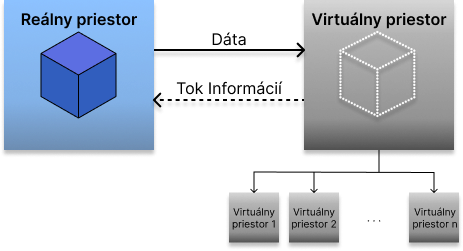
\includegraphics[width=0.8\linewidth]{assets/images/Grieves_PLM_model.png}
    \caption[Model zrkadlených priestorov]{Model zrkadlených priestorov (Mirrored Spaces Model) tak, ako ho vo svojej práci navrhol Grieves \cite{Grieves}. Tento model sa skladá z troch komponentov - reálny priestor (Real Space), virtuálny priestor (Virtual space) a spájací mechanizmus (Linking Mechanism) \cite{DT:OriginToFuture}, ktorý prúdi automatizovane oboma smermi medzi týmito priestormi. Virtuálny priestor vytvára digitálnu reprezentáciu reálnych objektov a podporuje viacero virtuálnych systémov na analýzu, simuláciu alebo predikciu správania fyzických objektov.}
    \label{fig:PLM}
\end{figure}

Vo  svojom výskume Enders a Hoßbachová \cite{DimensionOfDTAplication} identifikovali sektory, kde je používanie DT najrozšírenejšie. Patria sem výroba \cite{manuf}, letecký priemysel \cite{aircraft}, energetika \cite{energy}, automobilový priemysel \cite{automotive}, námorníctvo \cite{marine}, petrochemický priemysel \cite{oil}, poľnohospodárstvo \cite{agriculture}, zdravotníctvo \cite{health}, verejný sektor \cite{education} a ťažba \cite{mining}.

Taktiež identifikovali tri hlavné využitia DT v týchto oblastiach \cite{AplicationsOfDT}: ovládanie, simulovanie a monitorovanie. To však nepokrýva všetky možnosti a spôsoby využitia. DT dnes nájde uplatnenie aj pri dizajnovaní, validácii, predchádzaní chýb, trénovaní a optimalizácii.

Vývoj DT je podporený množstvom softvérových nástrojov líšiacich sa funkcionalitou a cenou. ANSYS Twin Builder je zameraný na presné fyzikálne modelovanie procesov (mechanika, elektromagnetizmus) a je vhodný pre tvorbu inžinierskych DT, pričom patrí medzi najnákladnejšie riešenia \cite{ansys_twin_builder}. Siemens MindSphere ponúka cloudovú platformu na správu dát a monitoring zariadení v priemyselných aplikáciách, s cenou závislou od rozsahu nasadenia \cite{siemens_mindsphere}. MATLAB a Simulink ponúkajú flexibilnú platformu pre tvorbu DT s dôrazom na simuláciu dynamických systémov, modelovanie riadiacich algoritmov a predikciu správania \cite{mathworks_digital_twin}.
Alternatívou bez licenčných nákladov je vlastná implementácia DT prostredí, kde je možné vytvoriť simulované kópie vybraných častí systému. Napríklad v oblasti 5G možno pomocou Open5GS a UERANSIM zostaviť základné virtuálne repliky siete, ktoré v kombinácii s vhodne naprogramovanými skriptami umožňujú budovanie DT.

Ak sa chceme pozrieť na reálne aplikácie DT, Huawei implementoval DT na monitorovanie výrobných liniek \cite{huawei2020}, zatiaľ čo mestá ako Bristol \cite{Bristol} či Singapur \cite{singapur} používajú DT na efektívne riadenie inteligentných mestských systémov. V týchto scenároch DT umožňuje predikciu zlyhaní, optimalizáciu zdrojov a minimalizáciu prestojov. 

V oblasti telekomunikácií umožňuje DT monitorovanie siete v reálnom čase, predikciu bezpečnostných incidentov a optimalizáciu konfigurácie bez zásahu do produkčnej infraštruktúry. Príkladom sú práce, ktoré implementovali DT do experimentálnych 5G jadier s cieľom analyzovať sieťové toky, detegovať anomálie a klasifikovať typ prevádzky pomocou strojového učenia \cite{DTof5G}.

Významnú úlohu tu zohráva výber príznakov, ktorý umožňuje redukovať výpočtovú náročnosť klasifikácie a zároveň zvyšuje robustnosť modelov v prostredí s vysokým objemom dát. Rôzne štúdie ukazujú, že výber príznakov výrazne ovplyvňuje výkon modelov najmä v prípade detekcie útokov distribuovaného odmietnutia služby (DoS) alebo neštandardného správania zariadení internetu vecí (IoT) v 5G jadre \cite{EffectiveFS}. Použité techniky zahŕňajú metódy ako Random Forest, k-najbližších susedov, rekurzívne odstraňovanie príznakov, permutačnú dôležitosť (PI) a ich kombinácie.

Z prehľadu literatúry vyplýva, že realistická simulácia sieťového správania a efektívna klasifikácia v reálnom čase si vyžadujú prepojenie viacerých nástrojov a metodík. Nasledujúca kapitola predstavuje konkrétny návrh a implementáciu DT systému, ktorý tieto poznatky aplikuje v kontexte 5G siete.


\section{Prehľad riešenia na vysokej úrovni}

Navrhnuté riešenie pozostáva z modulárneho systému na báze DT, ktorého cieľom je analyzovať a klasifikovať správanie 5G siete v kontrolovanom prostredí. Vytvorené DT simuluje vybrané komponenty reálnej siete a umožňuje generovanie syntetických dát, ich zber, spracovanie a následnú aplikáciu modelov strojového učenia. Architektúra systému bola navrhnutá s dôrazom na rozšíriteľnosť, modularitu a experimentálnu reprodukovateľnosť.

Open5GS je open-source implementácia 5G jadra siete, ktorá slúži ako základná riadiaca infraštruktúra pre prichádzajúce spojenia. V navrhnutom riešení zodpovedá za autentifikáciu zariadení, správu session a prideľovanie IP adries.

UERANSIM je emulátor RAN prístupu, ktorý generuje simulovaných používateľov (UE), ktorí sa pripájajú do siete (pozri Obr. \ref{fig:architecture}) cez definované scénare. Umožňuje flexibilne konfigurovať počet zariadení, typy prevádzky a časovanie spojení.

\begin{figure}[H]
    \centering
    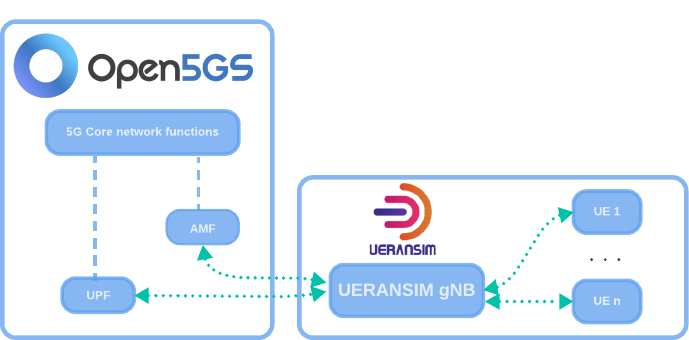
\includegraphics[width=0.75\linewidth]{assets//images/core-ue.png}
    \caption[Architektúra komponentov Open5GS a UERANSIM]{Architektúra jednotlivých komponentov Open5GS a UERANSIM a ich vzájomné prepojenie. Open5GS je rozdelené na riadiacu rovinu a rovinu užívateľských dát a obe tieto roviny sú napojené na gNB, ku ktorým sa môžu pripájať zariadenia.}
    \label{fig:architecture}
\end{figure}

Monitorovacia infraštruktúra pozostáva z nástrojov Prometheus, Grafana, Promtail a logwatcher.py. Prometheus zberá metriky zo siete a systémových zdrojov, ktoré sú vizualizované pomocou Grafany. Logwatcher je vlastný Python skript, ktorý analyzuje logy z Open5GS a exportuje vlastné metriky ako napr. počet aktívnych UE či SUCI identifikátory.

Skripty na simuláciu scenárov (UC) slúžia na spúšťanie preddefinovaných testovacích situácií. Každý UC definuje počet zariadení, objem prenesených dát a časovanie spojení, čím vytvára realistické syntetické zaťaženie siete.

Predspracovanie dát a výber metrík (EDA, preprocessing, feature selection) boli vykonané raz pred trénovaním modelu, s cieľom optimalizovať vstup pre model strojového učenia. Výber metrických premenných bol podporený metódami založenými na rozhodovacích stromoch a permutačnej dôležitosti.

Modely strojového učenia boli implementované pomocou LSTM modelov, ktoré sú vhodné pre sekvenčné dáta. Model bol natrénovaný na syntetických dátach a neskôr testovaný na dátach z reálnej siete.

\begin{figure}[H]
    \centering
    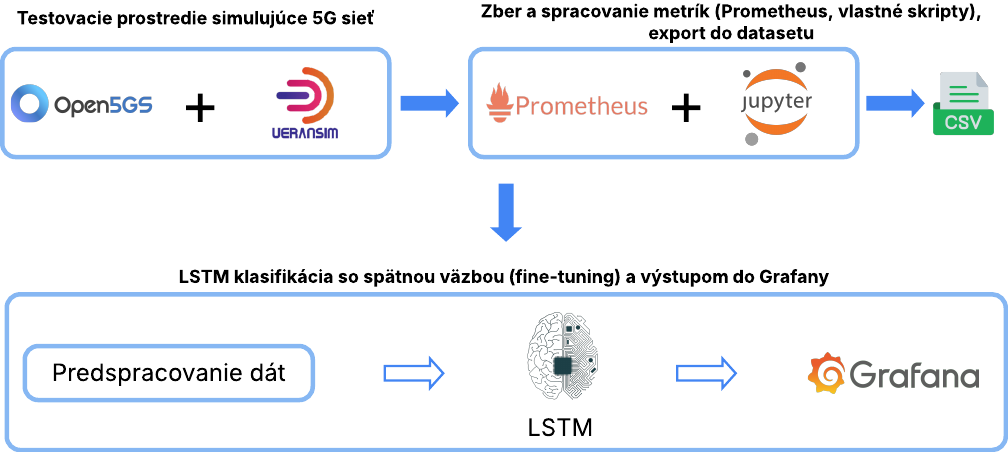
\includegraphics[width=0.95\linewidth]{assets//images/arch2.png}
    \caption[Architektúra systému: simulácia 5G siete, zber metrických dát a real-time klasifikácia s výstupom do Grafany.]{Zariadenia generované pomocou UERANSIM sa pripájajú k jadru siete v Open5GS, ktoré loguje udalosti a vystavuje metriky. Tieto údaje sú zbierané pomocou Promethea a logwatcher.py skriptu. Výstupy sú agregované do datasetu, ktorý sa ďalej spracúva v prostredí Jupyter Notebook. Po spracovaní sa dáta využívajú na trénovanie a testovanie modelov strojového učenia. Vizualizácia metrických údajov prebieha súbežne v Grafane.}
    \label{fig:arch}
\end{figure}

Modularita kontajnerizovaného riešenia založeného na Docker Compose umožňuje jednoduché nasadenie a replikáciu prostredia. Open-source komponenty boli zvolené kvôli dostupnosti a možnosti detailnej konfigurácie siete. Použitie syntetických scenárov poskytuje kontrolu nad testovaným správaním bez rizika ovplyvnenia reálnej prevádzky. LSTM siete boli zvolené vďaka schopnosti modelovať časové závislosti, ktoré sú kľúčové pri klasifikácii sieťového správania. Kombinácia reálneho a syntetického vstupu umožňuje overiť možnosti generalizácie modelov v telekomunikačnom prostredí.
 
\section{Hodnotenie rizík}
Implementácia digitálneho dvojčaťa 5G siete v kombinácii s klasifikačným modelom umelej inteligencie prináša niekoľko potenciálnych rizík, ktoré by mohli ovplyvniť presnosť, stabilitu a praktickú využiteľnosť riešenia \cite{ML_traffic}.

Jedným z najvýznamnejších rizík je nedostatočná kvalita vstupných dát. Vzhľadom na to, že systém sa bude spoliehať na syntetické metriky generované v simulovanom prostredí, existuje riziko, že tieto dáta nebudú dostatočne reprezentatívne pre správanie reálnej siete. To by mohlo negatívne ovplyvniť schopnosť modelu generalizovať. Ako mitigácia sa predpokladá testovanie viacerých variantov simulácií, aplikácia metód validácie \cite{Nguyen} (napr. krížová validácia) a neskôr prípadné doplnenie reálnych dátových vstupov \cite{data_generating}.

Ďalším rizikom je obmedzený čas dostupný na zber a spracovanie dát. Experimentálne simulácie si vyžadujú značné množstvo iterácií a manuálnej prípravy scenárov, čo môže limitovať rozsah a kvalitu datasetu pre modelovanie \cite{USAirForce}. Mitigáciou je dôsledné plánovanie simulácií, skriptovanie opakovaných činností a prioritizácia najrelevantnejších scenárov.

V oblasti softvérovej architektúry je potrebné počítať s možnou nekompatibilitou medzi jednotlivými komponentmi ako Open5GS, UERANSIM, Prometheus, Docker a vlastné skripty. Vzhľadom na to, že ide o open-source riešenia vyvíjané nezávisle, ich integrácia môže byť nestabilná alebo nedostatočne zdokumentovaná \cite{challenges_human_factor}. Navrhovanou stratégiou je modulárne nasadzovanie systémov, priebežné testovanie a dôsledná kontrola konfigurácií v menších izolovaných častiach.

Riziko predstavuje aj nedostatočná synchronizácia časových pečiatok medzi komponentmi, čo môže ovplyvniť presnosť dátových okien pre LSTM model. Tento problém je možné mitigovať precíznym logovaním timestampov a synchronizáciou systémového času medzi kontajnermi.

Z pohľadu bezpečnosti a etiky sa pri použití simulovanej siete s fiktívnymi údajmi a v uzavretom prostredí eliminuje riziko úniku osobných údajov či konfiguráčných súborov. Napriek tomu je vhodné minimalizovať citlivosť konfigurácií pomocou .env súborov \cite{Dt_Iot_data_worry_about} a testovať výhradne na syntetických identitách a IMSI.


\section{Technická reprodukovateľnosť a integrácia}

Riešenie DT 5G siete bolo vyvinuté s dôrazom na experimentálnu reprodukovateľnosť a jednoduché nasadenie. Celý projekt je dostupný vo verejnom repozitári na platforme GitHub\footnote{\url{https://github.com/xtruhlar/5GDigitalTwin}}, vrátane kompletného zdrojového kódu, Docker konfigurácie a skriptov pre klasifikáciu.

K spusteniu základného systému stačí klonovanie repozitára pomocou \texttt{git clone}, pričom je potrebné, aby bol na cieľovom systéme nainštalovaný  Git (2.39.5) a  Docker (28.0.1). Všetky závislosti sú zabudované do kontajnerov a celý systém je orchestrovaný pomocou \texttt{docker compose}. Po nakonfigurovaní premenných prostredia v súbore \texttt{.env} a inicializácii MongoDB databázy s preddefinovanými UE, sa systém spustí jedným príkazom:

\begin{quote} \texttt{docker compose -f deploy-all.yaml up --build -d} \end{quote}

Po nasadení komponentov je možné cez webové rozhranie Open5GS (port 9999) overiť funkčnosť jadra siete a cez Grafanu (port 3000) vizualizovať stav siete v reálnom čase. Konfigurácia UERANSIM gNB a UE je súčasťou repozitára a umožňuje simuláciu dynamického sieťového zaťaženia.

\subsection*{Zber dát}

Zber dát pre trénovanie a testovanie klasifikačných modelov bol realizovaný samostatne pre syntetickú a reálnu prevádzku. V prípade syntetických dát boli experimenty plne automatizované: systém bežal v Docker Compose prostredí. Skript každú sekundu extrahoval metriky z nástroja Prometheus, údaje z logov Open5GS a informácie o práve aktívnom UC zo sprievodného súboru. Každý riadok dát tak obsahoval časovú pečiatku, sieťové metriky, informácie o logoch a aktuálne označenie podľa spusteného UC.

Pri zbere reálnych dát bola situácia odlišná. Merania prebiehali v laboratórnom prostredí so skutočnými zariadeniami pripojenými do nezávislej 5G siete. Presný čas začiatku a konca každého používateľského scenára bol zaznamenaný manuálne. Po experimente boli všetky relevantné logy skopírované a vložené do preddefinovanej zložky, ktorú čítal ten istý skript. Na základe časového okna experimentu boli metriky zozbierané z Promethea a synchronizované s logmi. Pridávanie stĺpca s číslom UC do jednotlivých riadkov prebiehalo podľa známeho začiatku a konca testovaného UC. Tým bola zabezpečená konzistentnosť medzi stavom siete a cieľovou premennou modelu.

Výsledné datasety boli pre každý experiment exportované vo formáte CSV, pričom štruktúra bola zhodná pre syntetické aj reálne dáta.

\subsection*{Trénovanie modelov a použitie výstupov}

Na zabezpečenie rovnakých výsledkov trénovania boli dodržané nasledovné podmienky:

\begin{itemize}
  \item vo všetkých notebookoch sú fixované počiatočné hodnoty (seed), veľkosť dávky (batchu), počet epôch, architektúra modelu a stratifikované rozdelenie datasetu,
  \item krok 1: spustenie \texttt{eda\_feature\_selection.ipynb}, ktorý vytvorí súbor \\ \texttt{selected\_features.json},
  \item krok 2: spustenie \texttt{dataset\_processing.ipynb}, ktorý vygeneruje \texttt{X\_scaled.npy}, \texttt{y\_labels.npy} a \texttt{scaler.joblib},
  \item krok 3: spustenie \texttt{lstm\_preprocessing.ipynb}, ktorý vytvára sekvencie a exportuje ich vo formáte \texttt{X\_train.npy}, \texttt{y\_train.npy}, \texttt{X\_test.npy}, \texttt{y\_test.npy},
  \item krok 4: trénovanie modelov pomocou \texttt{lstm\_*\_model.ipynb} \\ (napr. \texttt{lstm\_attention\_model.ipynb}) na syntetických dátach,
  \item krok 5: vyhodnotenie na reálnych dátach v \texttt{eval\_results\_real\_data.ipynb},
\end{itemize}

Predtrénované modely sú uložené v \\ \texttt{/5GDigitalTwin/Implementation/data/Model/trained\_models}.

\subsection*{Klasifikácia v reálnom čase a ladenie modelu}

Kľúčovým komponentom riešenia je vlastný skript \texttt{network\_watcher.py}, ktorý slúži nielen na spracovanie logov z Open5GS, ale aj na priebežnú predikciu aktuálneho UC pomocou LSTM modelu a jeho ladenia na najnovších dátach. Skript beží ako samostatný proces v jednom z Docker kontajnerov a je automaticky spúšťaný pri štarte systému.

Každú sekundu skript načíta nové riadky z logov pomocou \texttt{pygtail}, extrahuje stav jednotlivých UE zariadení (registrácia, deregistrácia, trvanie relácií) a z týchto údajov vypočítava vlastné metriky. Zároveň načíta posledných 60 záznamov z generovaného CSV súboru, normalizuje ich, a použije ako vstup do už natrénovaného LSTM modelu. Výsledná predikcia je exportovaná ako vlastná Prometheus metrika spolu s pravdepodobnosťou predikovanej triedy (confidence score) a stratou (loss) počas tréningu.

\subsection*{Simulácia prípadov použitia}

Na automatizovanú simuláciu UC bol vytvorený skript \texttt{running\_network.py}, ktorý náhodne vyberá a spúšťa jednotlivé scenáre zo súborov \texttt{uc1.py} až \texttt{uc6.py}. Každý z týchto šiestich skriptov reprezentuje špecifický typ zaťaženia 5G siete, ako napríklad opakovanú registráciu používateľov, sťahovanie veľkého objemu dát, dlhodobé pripojenie s minimálnou aktivitou či anomálnu autentizáciu.

Skript \texttt{running\_network.py} funguje ako orchestrátor – každých niekoľko minút náhodne vyberie niektorý z UC skriptov, spustí ho v pozadí ako samostatný proces a následne ho po skončení ukončí. Informáciu o aktuálne bežiacom scenári zapisuje do súboru, ktorý slúži ako jediný zdroj pravdy pre označovanie zberaných metrických dát počas trvania experimentu.

Každý \texttt{ucX.py} skript (kde \( X \in \{1, \dots, 6\} \)) obsahuje definíciu počtu zariadení, konfiguráciu ich sieťového zaťaženia a dĺžku trvania simulácie. Scenáre boli navrhnuté tak, aby pokrývali reprezentatívne prípady bežnej aj abnormálnej prevádzky v 5G sieti. Táto architektúra umožňuje nielen spoľahlivý zber syntetických dát, ale aj jednoduché rozšírenie systému o ďalšie prípady použitia bez zásahu do zvyšku infraštruktúry.

Celá infraštruktúra tak poskytuje replikovateľné, modulárne a škálovateľné prostredie vhodné na výskum DT v oblasti 5G, s podporou klasifikácie, monitorovania a experimentálnej validácie modelov v reálnom čase.

\section{Udržateľnosť a environmentálny dopad}
%Študenti by mali opísať, ako by implementovali opatrenia na zabezpečenie udržateľnosti svojho produktu alebo služby počas životného cyklu. | 1-2 strany
Implementácia opatrení na zabezpečenie udržateľnosti projektu a minimalizácia jeho environmentálneho dopadu sú kľúčové pre zaistenie dlhodobej hodnoty, spoločenského prínosu a efektivity vypracovania tejto práce. Práca je navrhnutá s dôrazom na efektívne využívanie zdrojov, udržateľný softvérový a hardvérový návrh a životný cyklus 5G siete, ktorý minimalizuje potrebu používania fyzických zdrojov.

Jednou z hlavných prínosov DT je možnosť predikcie a optimalizácie, pričom ak je DT zostrojené správne, môže dopomôcť k redukcií spotreby elektrickej energie. \cite{DT_edge_networks_IoT}. Predikcia budúceho stavu siete umožňuje taktiež lepšiu správu záťaže (traffic load) a preťaženia (congestion), čo napomáha k znižovaniu nadmernej spotreby energie \cite{malaysia_enviro}. Navyše, DT eliminuje potrebu testovania na fyzických zariadeniach, čím sa minimalizuje spotreba rôznych materiálov \cite{enviro_raw_materials} a času potrebného na fyzické experimenty. Tento prístup je obzvlášť užitočný v prípade nasadzovania a testovania 5G technológií v oblastiach s nerozvinutou infraštruktúrou a obmedzenými výrobnými zdrojmi \cite{huaweii_i_cities}.

Vývoj softvéru bol orientovaný na maximálnu efektivitu, čo zahŕňa optimalizáciu kódu na zníženie spotreby energie počas behu aplikácie a nasadenie projektu v prostredí Docker, čo umožňuje rýchlejšiu konfiguráciu a škálovateľnosť zariadení. Tieto opatrenia nielen znižujú environmentálny dopad \cite{docker_enviro}\cite{docker_enviro_2}, ale aj zvyšujú celkovú udržateľnosť projektu.

Modulárny dizajn \cite{modular_sw} projektu zabezpečuje, že aktualizácie a údržba nemajú vplyv na celkovú funkčnosť systému. Tento prístup znižuje potrebu kompletného prekonfigurovania alebo fyzických zásahov do chodu programu, čo prispieva k dlhodobej udržateľnosti. Takýto dizajn môže mať pozitívny vplyv na životné prostredie \cite{modular_sw} (Green Design).

Ako je vyššie uvedené, použitie prediktívnych modelov v DT môže viesť k zásadným environmentálnym prínosom \cite{enviro}. Okrem zníženia zaťaženie fyzickej infraštruktúry a menej častých aktualizácie fyzického hardvéru, môže mať za následok aj nižšiu spotrebu zdrojov a menšiu produkciu odpadu \cite{enviro_raw_materials}. Predikčné modely teda umožňujú efektívnejšie rozhodovanie s pozitívnym dopadom na životné prostredie.

\section{Zamestnateľnosť}
Táto bakalárska práca, zameraná na rozvoj teoretických znalostí v oblasti DT v spojení s praktickou implementáciou a optimalizáciou 5G sietí, vedie k rozšíreniu zručností vo viacerých kľúčových oblastiach technologického sektora. V neposlednom rade strojové učenie, použité na klasifikáciu stavu implementovaného DT, zasahuje aj do oblasti dátovej vedy.

Vďaka formátu práce autori prejdú celým cyklom realizácie projektu, od prieskumu technológií cez návrh až po implementáciu a testovanie. Týmto získajú ucelený a komplexný pohľad na vývoj a riadenie softvérových projektov, ako aj na plánovanie, organizáciu a efektívnu komunikáciu.

Takáto kombinácia technických, projektových a komunikačných schopností môže významne zvýšiť hodnotu autorov na trhu práce, najmä v budúcnosti, keďže problematika DT a 5G sietí je stále viac žiadaná a nachádza uplatnenie v rôznych odvetviach.

\section{Tímová práca, diverzita a inklúzia}
%\par{
%Ak sa na projekte podieľajú odborníci z viacerých odborov, študent by mal implementovať procesy a opísať techniky pre zdieľanie úloh a (pochopenie) znalostí medzi rôznymi stranami. Mali by sa opísať problémy a stratégie na ich zmiernenie, aby sa zabezpečilo dokončenie projektu v stanovenom časovom harmonograme. Táto časť by mala obsahovať aj úvahy o diverzite a inklúzii. | ½-1 strana
%}
Na vypracovaní tejto bakalárskej práce som síce pracoval samostatne, no viaceré časti riešenia by neboli realizovateľné bez odbornej podpory a spolupráce s ďalšími osobami a komunitami.

Počas celého vývoja som úzko spolupracoval so školiteľom Ing. Matejom Petríkom, ktorý mi poskytol dôležité usmernenia v oblasti návrhu experimentov, spracovania dát a validácie výsledkov. V technických otázkach týkajúcich sa 5G sietí, konfigurácie Open5GS a správneho zberu metrických údajov zo siete som mal možnosť konzultovať s Ing. Matejom Janebom, ktorý sa aktívne podieľal na overovaní konfigurácie experimentálnej infraštruktúry a asistoval aj pri vytváraní reálneho datasetu v kontrolovanom laboratórnom prostredí.

Dôležitou súčasťou riešenia bola aj interakcia s komunitou vývojárov open-source nástroja UERANSIM. V rámci otvorenej komunikácie som kontaktoval hlavného autora projektu Aliho Güngöra so žiadosťou o objasnenie spracovania RRC Release signálov, ktoré v oficiálnej verzii nástroja absentovali. Tento typ spolupráce prispel k lepšiemu pochopeniu limitov dostupných nástrojov a ukázal význam komunitne vyvíjaného softvéru pri budovaní výskumných riešení.

Práca zohľadňuje princípy inklúzie tým, že všetky skripty a výstupy sú dokumentované, konfigurovateľné a prístupné pre širšiu výskumnú komunitu bez obmedzenia technologickej platformy či licencie. Prostredníctvom modularity riešenia, dôrazu na open-source a dokumentovanej kontajnerizácie je výstup tejto práce plne replikovateľný a využiteľný aj pre iných výskumníkov s rôznym zázemím a úrovňou odbornosti.


\chapter{Záver}

V rámci tejto bakalárskej práce bol navrhnutý a implementovaný základný model digitálneho dvojčaťa (DT) pre 5G sieť, ktorý umožňuje simuláciu správania siete a zber dát z fyzickej i simulovanej infraštruktúry. Použitím nástrojov Open5GS a UERANSIM bol vytvorený kontrolovaný experimentálny priestor, v ktorom bolo možné testovať rôzne používateľské scenáre bez zásahu do reálnej siete. Výsledky však ukazujú, že samotné Open5GS metriky zo simulovaného prostredia nie sú postačujúce na vytvorenie klasifikačného modelu, ktorý by spoľahlivo identifikoval správanie v reálnej 5G sieti. Modely trénované výhradne na syntetických dátach dosahovali výrazne horšiu presnosť pri testovaní na reálnych dátach (~16\%), čo poukazuje na značné rozdiely medzi simulovaným a skutočným sieťovým správaním. Táto skutočnosť zároveň poukazuje na potrebu pokročilejších metód prepojenia medzi syntetickými a reálnymi dátami.

Tieto zistenia poukazujú na viaceré limity implementovaného prístupu, ktoré je potrebné otvorene pomenovať. V prvom rade sa ukázalo, že syntetické metriky generované pomocou Open5GS majú obmedzenú schopnosť zachytiť komplexitu reálneho sieťového správania. Chýba im detailná reprezentácia QoS mechanizmov, realistický prenos na aplikačnej vrstve, ako aj podpora mobility, čo výrazne znižuje použiteľnosť týchto simulácií ako základ pre trénovanie modelov s dobrou generalizačnou schopnosťou. Hoci boli testované viaceré architektúry klasifikačných modelov (vrátane attention mechanizmu a batch normalizácie), výkonnosť na reálnych dátach ostávala nízka, čo naznačuje, že problém spočíva predovšetkým v obmedzenej kvalite dát. Navyše, použité metriky sa týkali výlučne core vrstvy, pričom chýbali detailnejšie údaje z RAN vrstvy, ako napríklad parametre rádiového signálu alebo využitie fyzických kanálov. Z pohľadu reálneho experimentálneho zberu bola práca obmedzená na malý počet zariadení, krátke trvanie meraní, čo mohlo ovplyvniť robustnosť výstupov. Hoci väčšina simulácií reprezentovala štandardné prípady správania, v jednom z prípadov bol zaradený aj anomálny scenár s odmietnutím pripojenia na základe neplatného IMSI, čo čiastočne zvýšilo rozmanitosť dát.

Výsledky tejto práce naznačujú, že DT môžu mať významné uplatnenie v oblasti riadenia a optimalizácie 5G sietí, predovšetkým ako nástroj na bezpečné testovanie sieťových zmien, včasné odhaľovanie anomálií a trénovanie systémov umelej inteligencie mimo produkčného prostredia. Do budúcnosti by mal byť výskum orientovaný na zvýšenie vernosti simulácií a zlepšenie kvality dát použitých na trénovanie modelov. Za účelom premostenia medzi syntetickými a reálnymi dátami sa ako perspektívna javí kombinácia metrických údajov z Open5GS s dátami zachytenými v podobe paketov (PCAP), čo umožní extrahovať dotatočné charakteristiky sieťového správania a vrstviť informácie naprieč L2–L7. Zároveň je potrebné preskúmať možnosti aplikácie pokročilých doménovo adaptačných techník, ktoré by mohli znížiť závislosť na rozsiahlych reálnych datasetoch.

Práca ukazuje, že real-time klasifikácia a online trénovanie modelov je technicky realizovateľné v rámci DT, hoci zatiaľ len pri použití syntetických dát. Výzvou do budúcnosti ostáva rozšíriť tento prístup aj na reálne sieťové prostredie a uzavrieť spätnú regulačnú slučku — teda umožniť systému nielen detegovať anomálie v reálnom čase, ale aj automaticky reagovať vhodnou rekonfiguráciou siete alebo notifikáciou správcu. Takýto obojsmerný tok dát medzi fyzickým a digitálnym prostredím predstavuje ďalší krok k autonómnym, adaptívnym sieťam piatej generácie. 
%\emptypage

\begin{comment}
\ifx\FIITlagEN\undefined
\else
% Resume in Slovak
\thispagestyle{empty}

\begin{otherlanguage}{slovak}
\chapter*{Resumé}
\markboth{Resumé}{Resumé}
\addcontentsline{toc}{chapter}{Resumé} 

\end{otherlanguage}

\fi
\end{comment}

% Bibliography
\printbibliography[heading=references,segment=\therefsegment]

% no page numbers for appendicies
\addtocontents{toc}{\protect\setcounter{tocdepth}{0}}
\addtocontents{toc}{\cftpagenumbersoff{chapter}}

%\emptypage

\end{refsegment}

% Appendix
\appendix

\setcounter{figure}{0}
\setcounter{listing}{0}

\chapter{Špecifikácia API rozhrania}
\label{appendix:API}
\pagenumbering{arabic}
\renewcommand*{\thepage}{A-\arabic{page}}

\begin{refsegment}

\par This is the application programming interface

\par \lipsum{10}

\section{Endpointy}

\begin{itemize}
  \item v1 - API version 1
  \item v2 - API version 2
  \item test - API placeholder
\end{itemize}

\section{Cesty}

\begin{itemize}
  \item \hyperref[section:auth]{A.2.1 Auth}
  \item \hyperref[section:music]{A.2.2 Music}
  \item \hyperref[section:pictures]{A.2.3 Pictures}
  \item \hyperref[section:video]{A.2.4 Video}
  \item \hyperref[section:mail]{A.2.5 Mail}
\end{itemize}

\subsection{Auth}
\label{section:auth}


\subsection{Music}
\label{section:music}


\subsection{Pictures}
\label{section:pictures}


\subsection{Video}
\label{section:video}


\subsection{Mail}
\label{section:mail}

% Bibliography
\printbibliography[heading=referencessec,segment=\therefsegment,resetnumbers=true]

\end{refsegment}

% Time schedule
\thispagestyle{empty}

\ifx\FIITlagEN\undefined
\chapter{Harmonogram práce}
\else
\chapter{Project task schedule}
\fi

\pagenumbering{arabic}
\renewcommand*{\thepage}{B-\arabic{page}}

\section{Zimný semester}

\begin{tabular}{|p{3cm}||p{10.2cm}|}
\hline
1. - 5. týždeň    & Konzultácie, rešerš problematiky  \\
\hline
6. týždeň    & Formulácia problému \\
\hline
7. týždeň   & Technický literárny prehľad \\
\hline
8. týždeň                       & Konzultovanie, Zamestnateľnosť   \\
\hline
9. - 10. týždeň   & Implementovanie pripomenutých zmien,  Hodnotenie rizík, Udržateľnosť a environmentálny dopad  \\
\hline
11. týždeň  & Návrh riešenia na vysokej úrovni \\
\hline
12. týždeň & Úvod, Konzultovanie, Implementovanie pripomenutých zmien, Odovzdávanie BP 1 \\
\hline
\end{tabular}

\subsection{Vyjadrenie k harmonogramu}
\par{
Harmonogram sa dodržal, čo prispelo k systematickému a plynulému postupu pri spracovaní bakalárskej práce. Pravidelné konzultácie s vedúcim práce zohrali kľúčovú úlohu pri jej realizácii. Vedúci poskytoval pripomienky a odporúčania, na základe ktorých sa jednotlivé časti práce mohli upraviť do súčasnej podoby. Tento proces mi umožnil efektívne riešiť prípadné nedostatky a zabezpečiť súčasnú kvalitu výsledného dokumentu.
}

\section{Letný semester - Predbežný plán}

\begin{tabular}{|p{3cm}||p{6.1cm}||p{4.1cm}|}
\hline
Týždeň & Bakalárska práca & Článok \\
\hline
1. - 2. týždeň & Tímová práca, diverzita a inklúzia, konzultovanie o implementácií & Related work  \\
\hline
3. - 4. týždeň & Open5GS, UERANSIM, srsRAN & Introduction, Methods, Index Terms \\
\hline
5. - 7.  týždeň  & Zber dát, Konfigurácia, MATLAB + Simulink & Data and Material  \\
\hline
8. - 10. týždeň & ML model, trénovanie, Experimentálna reprodukovateľnosť a integrácia & About author, Discussion  \\
\hline
11. týždeň & Konzultovanie, implementácie pripomienkovaných zmien, technický abstrakt, laický abstrakt & Results, Abstract, Lay abstract  \\
\hline
12. týždeň &  Zhrnutie, úpravy, konzultovanie & Conclusion, Future work \\
\hline
\end{tabular}


%% Contents of the digital medium
\thispagestyle{empty}

\ifx\FIITlagEN\undefined
\chapter{Obsah digitálneho média}
\else
\chapter{Contents of the digital medium}
\fi

\pagenumbering{arabic}
\renewcommand*{\thepage}{C-\arabic{page}}

\ifx\FIITlagEN\undefined
\par Evidenčné číslo práce v informačnom systéme: \FIITevidenceNumber
\else
\par Registration number of the thesis in the information system: \FIITevidenceNumber
\fi

\ifx\FIITlagEN\undefined
\par Obsah digitálnej časti práce (archív ZIP):
\else
\par Contents of the digital medium (ZIP archive):
\fi

\begin{minted}[linenos=false]{text}
Folder                  Contents
/bin                    binárne súbory umožňujúce ...
    /service
    /app
/models                 modely opísané v práci
    modelA
    modelB
/scripts
/data                   dátové množiny použité na ...
/praca-pdf              pdf verzia záverečnej práce
    /praca.pdf          pdf hlavná časť záverečnej práce
    /prilohy.pdf        pdf textové prílohy záverečnej práce

\end{minted}

% only if digital medium contents exceed 1 GB
% \par Digitálna časť práce má veľkosť 3.75 GB, kvôli čomu je uložená v systéme G Suite for Education.


\ifx\FIITlagEN\undefined
\par Názov odovzdaného archívu: \FIITArchiveName.
\else
\par Name of the submitted archive: \FIITArchiveName.
\fi


\end{document}
